% =============================================================================
% chapters/ch04_quant_main.tex — Quantitative core (the empirical burden)
% Pulled into manuscript.tex via % =============================================================================
% chapters/ch04_quant_main.tex — Quantitative core (the empirical burden)
% Pulled into manuscript.tex via % =============================================================================
% chapters/ch04_quant_main.tex — Quantitative core (the empirical burden)
% Pulled into manuscript.tex via % =============================================================================
% chapters/ch04_quant_main.tex — Quantitative core (the empirical burden)
% Pulled into manuscript.tex via \include{chapters/ch04_quant_main}.
%
% This chapter carries the dissertation's empirical weight (the qualitative case
% chapters were dropped). Every number here must trace to an R pipeline under
% Dissertation/analyses/NN/. Wiring convention:
%   - Table fragments:  \input{tables/<name>.tex}
%     produced by analyses/01_quant_main/scripts/R/04_tables.R, then copied/
%     written into Dissertation/tables/.
%   - Inline numbers:   annotate with  %% source: analyses/NN/scripts/R/03_analyze.R
%     so /audit-reproducibility can check the paper<->code graph.
% =============================================================================
\chapter{Aid Competition across Spheres of Influence: Quantitative Evidence}
\label{ch:quant}

\textit{Placeholder.} The empirical core. Short-run allocation models by region,
an instrumental-variables strategy for Chinese aid exposure, and a long-run
dynamics test establish whether US and Chinese aid race or diverge across
contested spheres.

\section{Data}
\label{sec:quant-data}
\textit{Placeholder.} AidData Global Chinese Development Finance (GCDF) for
Chinese official finance; OECD-DAC Creditor Reporting System (CRS) for US and
other DAC aid. Unit of analysis: recipient-country $\times$ year. Sample period,
coverage, and the sphere-of-influence covariates defined in
Chapter~\ref{ch:theory}.

\section{Empirical strategy}
\label{sec:quant-strategy}
\textit{Placeholder.} Short-run allocation model with country and year fixed
effects; identification concerns; the Dreher/Zeitz-style shift-share instrument
(Chinese steel production $\times$ recipient exposure) developed in
\texttt{analyses/03\_iv\_robustness/}; and the panel-VAR / Granger test of
long-run co-evolution in \texttt{analyses/04\_var\_dynamics/}.

\section{Results}
\label{sec:quant-results}
\textit{Placeholder.} Main short-run results table:

% \input{tables/table_main.tex}     %% source: analyses/01_quant_main/scripts/R/04_tables.R

\textit{Placeholder.} Report the headline pattern here once the pipeline is run:
a positive US--China aid correlation in Africa
(prospectus: $+0.113$)                                %% source: analyses/01_quant_main/scripts/R/03_analyze.R
and negative correlations outside Africa, consistent with H1.

\section{Instrumental-variables robustness}
\label{sec:quant-iv}
\textit{Placeholder.} IV estimates and first-stage diagnostics:

% \input{tables/table_iv.tex}       %% source: analyses/03_iv_robustness/scripts/R/04_tables.R

\section{Long-run dynamics}
\label{sec:quant-var}
\textit{Placeholder.} Panel-VAR impulse responses / Granger-causality:

% \input{tables/table_var.tex}      %% source: analyses/04_var_dynamics/scripts/R/04_tables.R
% 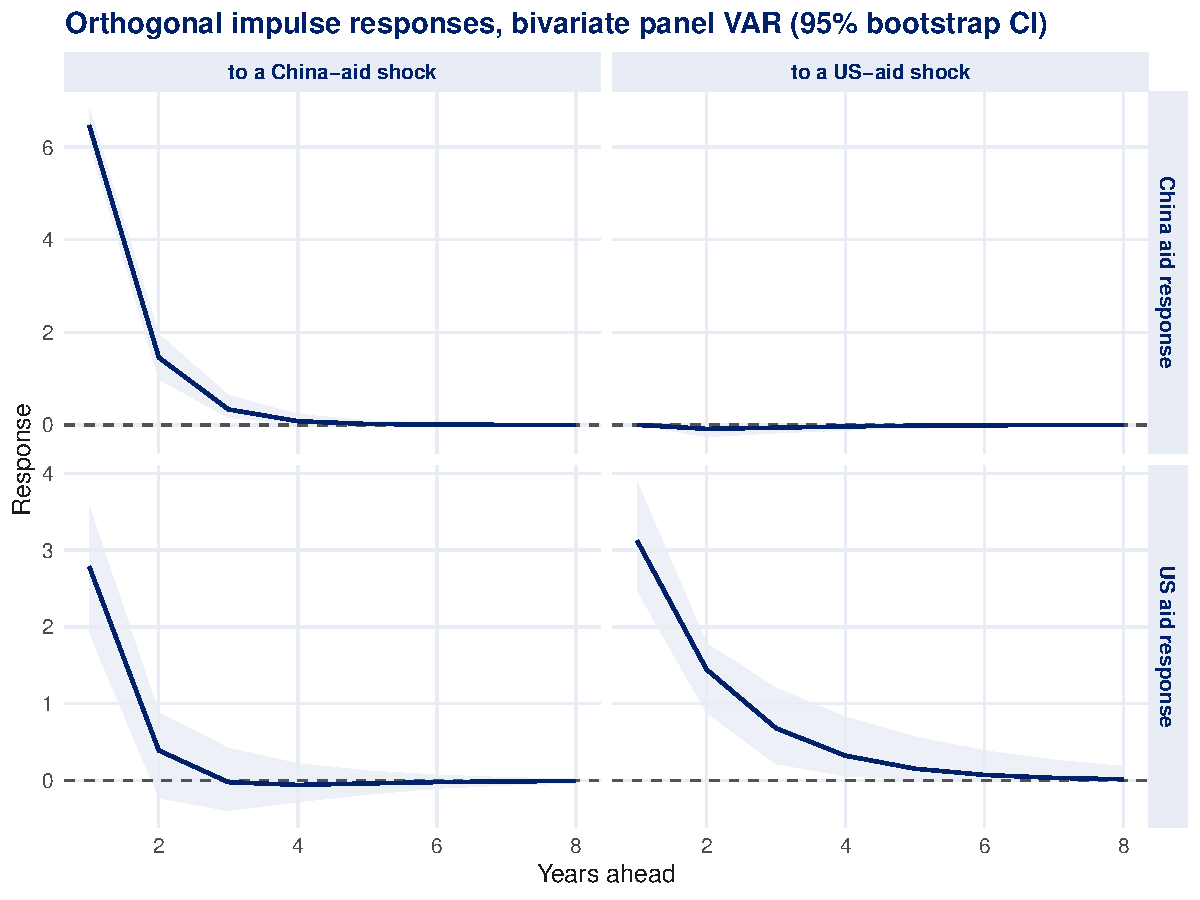
\includegraphics{fig_irf}         %% source: analyses/04_var_dynamics/scripts/R/05_figures.R

\section{Robustness}
\label{sec:quant-robustness}
\textit{Placeholder.} Specification curve / multiverse, leave-one-out by region,
alternative clustering and inference (per the project's inference-robustness
conventions).
.
%
% This chapter carries the dissertation's empirical weight (the qualitative case
% chapters were dropped). Every number here must trace to an R pipeline under
% Dissertation/analyses/NN/. Wiring convention:
%   - Table fragments:  \input{tables/<name>.tex}
%     produced by analyses/01_quant_main/scripts/R/04_tables.R, then copied/
%     written into Dissertation/tables/.
%   - Inline numbers:   annotate with  %% source: analyses/NN/scripts/R/03_analyze.R
%     so /audit-reproducibility can check the paper<->code graph.
% =============================================================================
\chapter{Aid Competition across Spheres of Influence: Quantitative Evidence}
\label{ch:quant}

\textit{Placeholder.} The empirical core. Short-run allocation models by region,
an instrumental-variables strategy for Chinese aid exposure, and a long-run
dynamics test establish whether US and Chinese aid race or diverge across
contested spheres.

\section{Data}
\label{sec:quant-data}
\textit{Placeholder.} AidData Global Chinese Development Finance (GCDF) for
Chinese official finance; OECD-DAC Creditor Reporting System (CRS) for US and
other DAC aid. Unit of analysis: recipient-country $\times$ year. Sample period,
coverage, and the sphere-of-influence covariates defined in
Chapter~\ref{ch:theory}.

\section{Empirical strategy}
\label{sec:quant-strategy}
\textit{Placeholder.} Short-run allocation model with country and year fixed
effects; identification concerns; the Dreher/Zeitz-style shift-share instrument
(Chinese steel production $\times$ recipient exposure) developed in
\texttt{analyses/03\_iv\_robustness/}; and the panel-VAR / Granger test of
long-run co-evolution in \texttt{analyses/04\_var\_dynamics/}.

\section{Results}
\label{sec:quant-results}
\textit{Placeholder.} Main short-run results table:

% \begin{table}[htbp]
\centering
\caption{Short-run US aid response to lagged Chinese finance, by region}
\label{tab:main}
\begin{tabular}{lcc}
\toprule
Region & China (all official finance) & China (ODA-like only) \\
\midrule
Pooled & 0.053*** & 0.046** \\
 & (0.019) & (0.019) \\
 & [N=3300, 150 ctry] & [N=3300, 150 ctry] \\[2pt]
Africa & 0.039 & 0.037 \\
 & (0.038) & (0.035) \\
 & [N=1188, 54 ctry] & [N=1188, 54 ctry] \\[2pt]
Americas & 0.046 & 0.023 \\
 & (0.033) & (0.039) \\
 & [N=770, 35 ctry] & [N=770, 35 ctry] \\[2pt]
Asia & 0.015 & 0.008 \\
 & (0.022) & (0.016) \\
 & [N=858, 39 ctry] & [N=858, 39 ctry] \\[2pt]
Europe & 0.229* & 0.156* \\
 & (0.110) & (0.078) \\
 & [N=242, 11 ctry] & [N=242, 11 ctry] \\[2pt]
Oceania & 0.061 & 0.081 \\
 & (0.067) & (0.075) \\
 & [N=242, 11 ctry] & [N=242, 11 ctry] \\[2pt]
\bottomrule
\end{tabular}
\begin{minipage}{0.9\textwidth}
\vspace{4pt}
\footnotesize Coefficient on log(lagged China finance + 1) from
log(US ODA + 1) $\sim$ log(China finance$_{t-1}$ + 1) with year and
country fixed effects; SEs clustered by country. * p<0.10, ** p<0.05, *** p<0.01.
\end{minipage}
\end{table}
     %% source: analyses/01_quant_main/scripts/R/04_tables.R

\textit{Placeholder.} Report the headline pattern here once the pipeline is run:
a positive US--China aid correlation in Africa
(prospectus: $+0.113$)                                %% source: analyses/01_quant_main/scripts/R/03_analyze.R
and negative correlations outside Africa, consistent with H1.

\section{Instrumental-variables robustness}
\label{sec:quant-iv}
\textit{Placeholder.} IV estimates and first-stage diagnostics:

% \begin{table}[htbp]
\centering
\caption{Shift-share IV for Chinese finance: first-stage diagnostics by share definition}
\label{tab:iv}
\small
\begin{tabular}{lcccc}
\toprule
Exposure share & 1st-stage coef. & 1st-stage $t$ & 1st-stage $F$ & 2SLS estimate \\
\midrule
Predetermined (1970--99) & -0.527 & -0.36 & 0.27 & -2.466 \\
 & & & & (7.648) \\[2pt]
Contemporaneous (2000--15) & 3.089 & 4.97 & 27.33 & 0.321 \\
 & & & & (0.247) \\[2pt]
\bottomrule
\end{tabular}
\begin{minipage}{0.92\textwidth}
\vspace{4pt}
\footnotesize Instrument $=\ln(\text{Chinese crude steel production}_{t-1})\times\text{exposure share}_i$,
following Dreher, Fuchs, Parks, Strange and Tierney (2021). Outcome is $\log(\text{US ODA}+1)$,
endogenous regressor $\log(\text{Chinese official finance}_{t-1}+1)$; year and country fixed
effects, SEs clustered by country. Sample 2000--2015 (bounded by the WSA steel series).
OLS on the same sample: $0.036$**. * p<0.10, ** p<0.05, *** p<0.01.
\textbf{Read this table as a diagnosis, not an estimate.} The predetermined share is the
methodologically valid one and produces no first stage. The contemporaneous share is
constructed from the same post-2000 Chinese-finance variation the instrument is meant to
purge, so its first-stage power is mechanical rather than evidence the design identifies
anything. Neither 2SLS column supports inference.
\end{minipage}
\end{table}
       %% source: analyses/03_iv_robustness/scripts/R/04_tables.R

\section{Long-run dynamics}
\label{sec:quant-var}
\textit{Placeholder.} Panel-VAR impulse responses / Granger-causality:

% \begin{table}[htbp]
\centering
\caption{Bivariate panel VAR: US and Chinese aid, 2000--2021 (system GMM)}
\label{tab:var}
\begin{tabular}{lccc}
\toprule
 & US aid (log, $t-1$) & China aid (log, $t-1$) & Constant \\
\midrule
US aid (log, $t$) & 0.475*** & -0.013 & 8.164*** \\
 & (0.110) & (0.016) & (1.748) \\[2pt]
China aid (log, $t$) & -0.075 & 0.225*** & 9.755*** \\
 & (0.129) & (0.048) & (2.124) \\[2pt]
\bottomrule
\end{tabular}
\begin{minipage}{0.9\textwidth}
\vspace{4pt}
\footnotesize Two-step system GMM, forward-orthogonal-deviations, collapsed
instruments; Windmeijer-corrected SEs in parens. * p<0.10, ** p<0.05, *** p<0.01.
Hansen J test of overidentifying restrictions: $\chi^2(28) = 100.22$, $p < 0.001$ --
\textbf{rejects} at conventional levels (34 instruments over 150 groups); interpret with caution.
Stability: companion-matrix eigenvalues all lie inside the unit circle.
\end{minipage}
\end{table}
      %% source: analyses/04_var_dynamics/scripts/R/04_tables.R
% 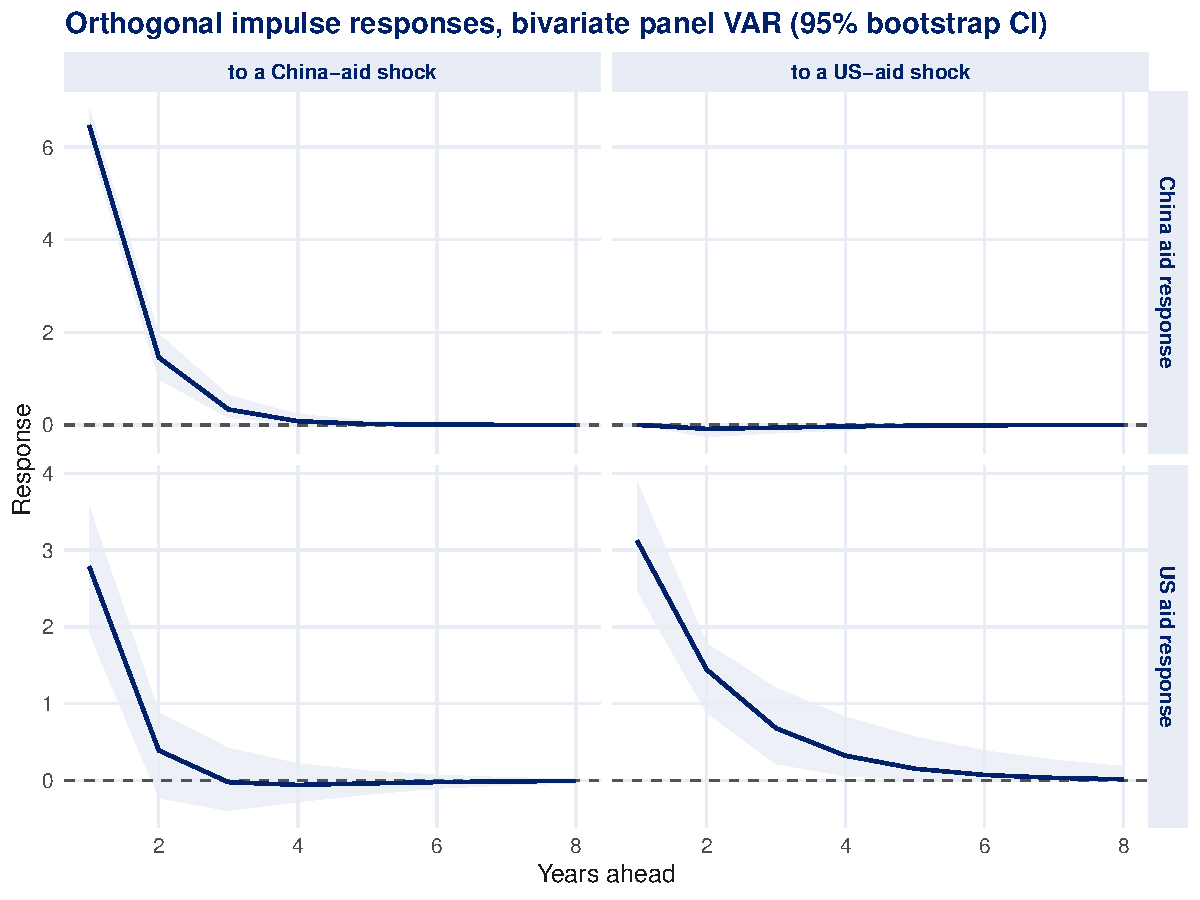
\includegraphics{fig_irf}         %% source: analyses/04_var_dynamics/scripts/R/05_figures.R

\section{Robustness}
\label{sec:quant-robustness}
\textit{Placeholder.} Specification curve / multiverse, leave-one-out by region,
alternative clustering and inference (per the project's inference-robustness
conventions).
.
%
% This chapter carries the dissertation's empirical weight (the qualitative case
% chapters were dropped). Every number here must trace to an R pipeline under
% Dissertation/analyses/NN/. Wiring convention:
%   - Table fragments:  \input{tables/<name>.tex}
%     produced by analyses/01_quant_main/scripts/R/04_tables.R, then copied/
%     written into Dissertation/tables/.
%   - Inline numbers:   annotate with  %% source: analyses/NN/scripts/R/03_analyze.R
%     so /audit-reproducibility can check the paper<->code graph.
% =============================================================================
\chapter{Aid Competition across Spheres of Influence: Quantitative Evidence}
\label{ch:quant}

\textit{Placeholder.} The empirical core. Short-run allocation models by region,
an instrumental-variables strategy for Chinese aid exposure, and a long-run
dynamics test establish whether US and Chinese aid race or diverge across
contested spheres.

\section{Data}
\label{sec:quant-data}
\textit{Placeholder.} AidData Global Chinese Development Finance (GCDF) for
Chinese official finance; OECD-DAC Creditor Reporting System (CRS) for US and
other DAC aid. Unit of analysis: recipient-country $\times$ year. Sample period,
coverage, and the sphere-of-influence covariates defined in
Chapter~\ref{ch:theory}.

\section{Empirical strategy}
\label{sec:quant-strategy}
\textit{Placeholder.} Short-run allocation model with country and year fixed
effects; identification concerns; the Dreher/Zeitz-style shift-share instrument
(Chinese steel production $\times$ recipient exposure) developed in
\texttt{analyses/03\_iv\_robustness/}; and the panel-VAR / Granger test of
long-run co-evolution in \texttt{analyses/04\_var\_dynamics/}.

\section{Results}
\label{sec:quant-results}
\textit{Placeholder.} Main short-run results table:

% \begin{table}[htbp]
\centering
\caption{Short-run US aid response to lagged Chinese finance, by region}
\label{tab:main}
\begin{tabular}{lcc}
\toprule
Region & China (all official finance) & China (ODA-like only) \\
\midrule
Pooled & 0.053*** & 0.046** \\
 & (0.019) & (0.019) \\
 & [N=3300, 150 ctry] & [N=3300, 150 ctry] \\[2pt]
Africa & 0.039 & 0.037 \\
 & (0.038) & (0.035) \\
 & [N=1188, 54 ctry] & [N=1188, 54 ctry] \\[2pt]
Americas & 0.046 & 0.023 \\
 & (0.033) & (0.039) \\
 & [N=770, 35 ctry] & [N=770, 35 ctry] \\[2pt]
Asia & 0.015 & 0.008 \\
 & (0.022) & (0.016) \\
 & [N=858, 39 ctry] & [N=858, 39 ctry] \\[2pt]
Europe & 0.229* & 0.156* \\
 & (0.110) & (0.078) \\
 & [N=242, 11 ctry] & [N=242, 11 ctry] \\[2pt]
Oceania & 0.061 & 0.081 \\
 & (0.067) & (0.075) \\
 & [N=242, 11 ctry] & [N=242, 11 ctry] \\[2pt]
\bottomrule
\end{tabular}
\begin{minipage}{0.9\textwidth}
\vspace{4pt}
\footnotesize Coefficient on log(lagged China finance + 1) from
log(US ODA + 1) $\sim$ log(China finance$_{t-1}$ + 1) with year and
country fixed effects; SEs clustered by country. * p<0.10, ** p<0.05, *** p<0.01.
\end{minipage}
\end{table}
     %% source: analyses/01_quant_main/scripts/R/04_tables.R

\textit{Placeholder.} Report the headline pattern here once the pipeline is run:
a positive US--China aid correlation in Africa
(prospectus: $+0.113$)                                %% source: analyses/01_quant_main/scripts/R/03_analyze.R
and negative correlations outside Africa, consistent with H1.

\section{Instrumental-variables robustness}
\label{sec:quant-iv}
\textit{Placeholder.} IV estimates and first-stage diagnostics:

% \begin{table}[htbp]
\centering
\caption{Shift-share IV for Chinese finance: first-stage diagnostics by share definition}
\label{tab:iv}
\small
\begin{tabular}{lcccc}
\toprule
Exposure share & 1st-stage coef. & 1st-stage $t$ & 1st-stage $F$ & 2SLS estimate \\
\midrule
Predetermined (1970--99) & -0.527 & -0.36 & 0.27 & -2.466 \\
 & & & & (7.648) \\[2pt]
Contemporaneous (2000--15) & 3.089 & 4.97 & 27.33 & 0.321 \\
 & & & & (0.247) \\[2pt]
\bottomrule
\end{tabular}
\begin{minipage}{0.92\textwidth}
\vspace{4pt}
\footnotesize Instrument $=\ln(\text{Chinese crude steel production}_{t-1})\times\text{exposure share}_i$,
following Dreher, Fuchs, Parks, Strange and Tierney (2021). Outcome is $\log(\text{US ODA}+1)$,
endogenous regressor $\log(\text{Chinese official finance}_{t-1}+1)$; year and country fixed
effects, SEs clustered by country. Sample 2000--2015 (bounded by the WSA steel series).
OLS on the same sample: $0.036$**. * p<0.10, ** p<0.05, *** p<0.01.
\textbf{Read this table as a diagnosis, not an estimate.} The predetermined share is the
methodologically valid one and produces no first stage. The contemporaneous share is
constructed from the same post-2000 Chinese-finance variation the instrument is meant to
purge, so its first-stage power is mechanical rather than evidence the design identifies
anything. Neither 2SLS column supports inference.
\end{minipage}
\end{table}
       %% source: analyses/03_iv_robustness/scripts/R/04_tables.R

\section{Long-run dynamics}
\label{sec:quant-var}
\textit{Placeholder.} Panel-VAR impulse responses / Granger-causality:

% \begin{table}[htbp]
\centering
\caption{Bivariate panel VAR: US and Chinese aid, 2000--2021 (system GMM)}
\label{tab:var}
\begin{tabular}{lccc}
\toprule
 & US aid (log, $t-1$) & China aid (log, $t-1$) & Constant \\
\midrule
US aid (log, $t$) & 0.475*** & -0.013 & 8.164*** \\
 & (0.110) & (0.016) & (1.748) \\[2pt]
China aid (log, $t$) & -0.075 & 0.225*** & 9.755*** \\
 & (0.129) & (0.048) & (2.124) \\[2pt]
\bottomrule
\end{tabular}
\begin{minipage}{0.9\textwidth}
\vspace{4pt}
\footnotesize Two-step system GMM, forward-orthogonal-deviations, collapsed
instruments; Windmeijer-corrected SEs in parens. * p<0.10, ** p<0.05, *** p<0.01.
Hansen J test of overidentifying restrictions: $\chi^2(28) = 100.22$, $p < 0.001$ --
\textbf{rejects} at conventional levels (34 instruments over 150 groups); interpret with caution.
Stability: companion-matrix eigenvalues all lie inside the unit circle.
\end{minipage}
\end{table}
      %% source: analyses/04_var_dynamics/scripts/R/04_tables.R
% 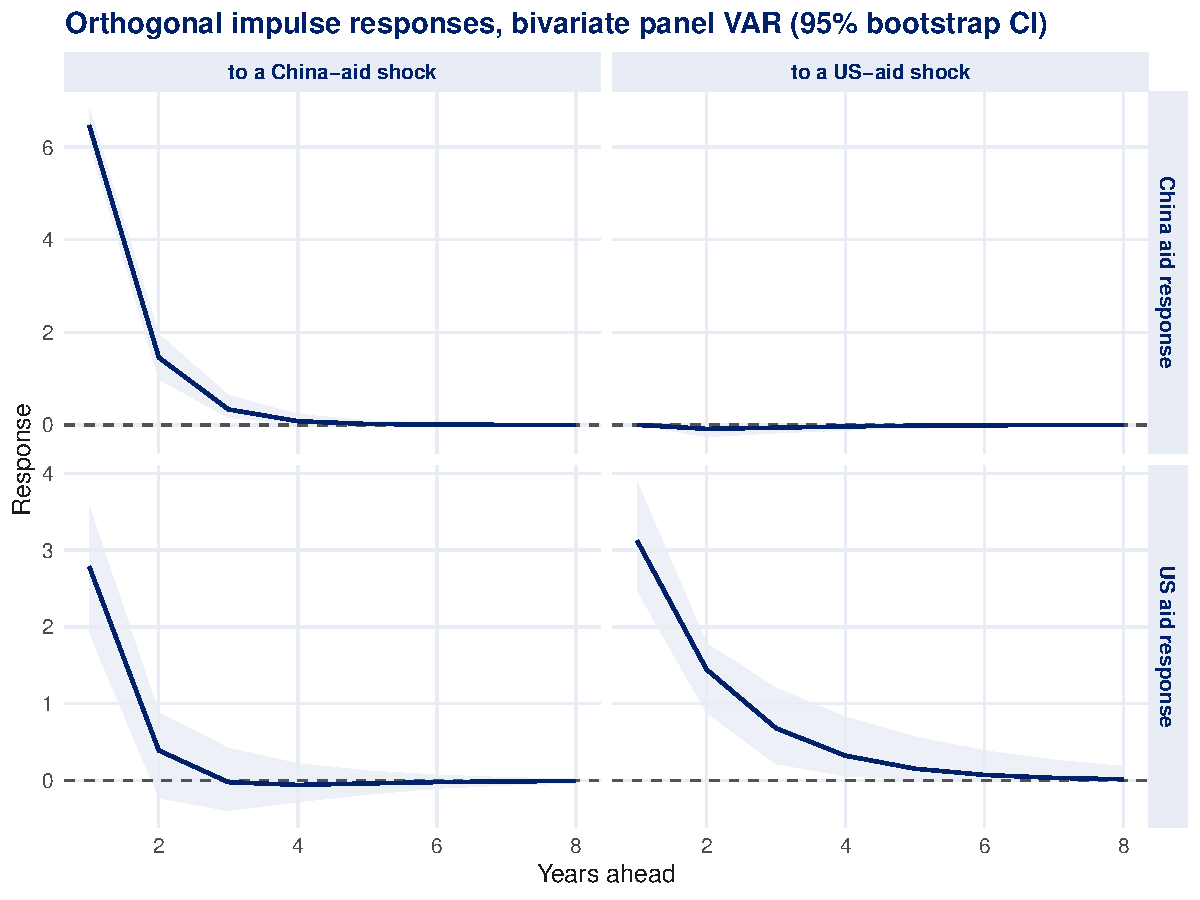
\includegraphics{fig_irf}         %% source: analyses/04_var_dynamics/scripts/R/05_figures.R

\section{Robustness}
\label{sec:quant-robustness}
\textit{Placeholder.} Specification curve / multiverse, leave-one-out by region,
alternative clustering and inference (per the project's inference-robustness
conventions).
.
%
% This chapter carries the dissertation's empirical weight (the qualitative case
% chapters were dropped). Every number here must trace to an R pipeline under
% Dissertation/analyses/NN/. Wiring convention:
%   - Table fragments:  \input{tables/<name>.tex}
%     produced by analyses/01_quant_main/scripts/R/04_tables.R, then copied/
%     written into Dissertation/tables/.
%   - Inline numbers:   annotate with  %% source: analyses/NN/scripts/R/03_analyze.R
%     so /audit-reproducibility can check the paper<->code graph.
% =============================================================================
\chapter{Aid Competition across Spheres of Influence: Quantitative Evidence}
\label{ch:quant}

\textit{Placeholder.} The empirical core. Short-run allocation models by region,
an instrumental-variables strategy for Chinese aid exposure, and a long-run
dynamics test establish whether US and Chinese aid race or diverge across
contested spheres.

\section{Data}
\label{sec:quant-data}
\textit{Placeholder.} AidData Global Chinese Development Finance (GCDF) for
Chinese official finance; OECD-DAC Creditor Reporting System (CRS) for US and
other DAC aid. Unit of analysis: recipient-country $\times$ year. Sample period,
coverage, and the sphere-of-influence covariates defined in
Chapter~\ref{ch:theory}.

\section{Empirical strategy}
\label{sec:quant-strategy}
\textit{Placeholder.} Short-run allocation model with country and year fixed
effects; identification concerns; the Dreher/Zeitz-style shift-share instrument
(Chinese steel production $\times$ recipient exposure) developed in
\texttt{analyses/03\_iv\_robustness/}; and the panel-VAR / Granger test of
long-run co-evolution in \texttt{analyses/04\_var\_dynamics/}.

\section{Results}
\label{sec:quant-results}
\textit{Placeholder.} Main short-run results table:

% \begin{table}[htbp]
\centering
\caption{Short-run US aid response to lagged Chinese finance, by region}
\label{tab:main}
\begin{tabular}{lcc}
\toprule
Region & China (all official finance) & China (ODA-like only) \\
\midrule
Pooled & 0.053*** & 0.046** \\
 & (0.019) & (0.019) \\
 & [N=3300, 150 ctry] & [N=3300, 150 ctry] \\[2pt]
Africa & 0.039 & 0.037 \\
 & (0.038) & (0.035) \\
 & [N=1188, 54 ctry] & [N=1188, 54 ctry] \\[2pt]
Americas & 0.046 & 0.023 \\
 & (0.033) & (0.039) \\
 & [N=770, 35 ctry] & [N=770, 35 ctry] \\[2pt]
Asia & 0.015 & 0.008 \\
 & (0.022) & (0.016) \\
 & [N=858, 39 ctry] & [N=858, 39 ctry] \\[2pt]
Europe & 0.229* & 0.156* \\
 & (0.110) & (0.078) \\
 & [N=242, 11 ctry] & [N=242, 11 ctry] \\[2pt]
Oceania & 0.061 & 0.081 \\
 & (0.067) & (0.075) \\
 & [N=242, 11 ctry] & [N=242, 11 ctry] \\[2pt]
\bottomrule
\end{tabular}
\begin{minipage}{0.9\textwidth}
\vspace{4pt}
\footnotesize Coefficient on log(lagged China finance + 1) from
log(US ODA + 1) $\sim$ log(China finance$_{t-1}$ + 1) with year and
country fixed effects; SEs clustered by country. * p<0.10, ** p<0.05, *** p<0.01.
\end{minipage}
\end{table}
     %% source: analyses/01_quant_main/scripts/R/04_tables.R

\textit{Placeholder.} Report the headline pattern here once the pipeline is run:
a positive US--China aid correlation in Africa
(prospectus: $+0.113$)                                %% source: analyses/01_quant_main/scripts/R/03_analyze.R
and negative correlations outside Africa, consistent with H1.

\section{Instrumental-variables robustness}
\label{sec:quant-iv}
\textit{Placeholder.} IV estimates and first-stage diagnostics:

% \begin{table}[htbp]
\centering
\caption{Shift-share IV for Chinese finance: first-stage diagnostics by share definition}
\label{tab:iv}
\small
\begin{tabular}{lcccc}
\toprule
Exposure share & 1st-stage coef. & 1st-stage $t$ & 1st-stage $F$ & 2SLS estimate \\
\midrule
Predetermined (1970--99) & -0.527 & -0.36 & 0.27 & -2.466 \\
 & & & & (7.648) \\[2pt]
Contemporaneous (2000--15) & 3.089 & 4.97 & 27.33 & 0.321 \\
 & & & & (0.247) \\[2pt]
\bottomrule
\end{tabular}
\begin{minipage}{0.92\textwidth}
\vspace{4pt}
\footnotesize Instrument $=\ln(\text{Chinese crude steel production}_{t-1})\times\text{exposure share}_i$,
following Dreher, Fuchs, Parks, Strange and Tierney (2021). Outcome is $\log(\text{US ODA}+1)$,
endogenous regressor $\log(\text{Chinese official finance}_{t-1}+1)$; year and country fixed
effects, SEs clustered by country. Sample 2000--2015 (bounded by the WSA steel series).
OLS on the same sample: $0.036$**. * p<0.10, ** p<0.05, *** p<0.01.
\textbf{Read this table as a diagnosis, not an estimate.} The predetermined share is the
methodologically valid one and produces no first stage. The contemporaneous share is
constructed from the same post-2000 Chinese-finance variation the instrument is meant to
purge, so its first-stage power is mechanical rather than evidence the design identifies
anything. Neither 2SLS column supports inference.
\end{minipage}
\end{table}
       %% source: analyses/03_iv_robustness/scripts/R/04_tables.R

\section{Long-run dynamics}
\label{sec:quant-var}
\textit{Placeholder.} Panel-VAR impulse responses / Granger-causality:

% \begin{table}[htbp]
\centering
\caption{Bivariate panel VAR: US and Chinese aid, 2000--2021 (system GMM)}
\label{tab:var}
\begin{tabular}{lccc}
\toprule
 & US aid (log, $t-1$) & China aid (log, $t-1$) & Constant \\
\midrule
US aid (log, $t$) & 0.475*** & -0.013 & 8.164*** \\
 & (0.110) & (0.016) & (1.748) \\[2pt]
China aid (log, $t$) & -0.075 & 0.225*** & 9.755*** \\
 & (0.129) & (0.048) & (2.124) \\[2pt]
\bottomrule
\end{tabular}
\begin{minipage}{0.9\textwidth}
\vspace{4pt}
\footnotesize Two-step system GMM, forward-orthogonal-deviations, collapsed
instruments; Windmeijer-corrected SEs in parens. * p<0.10, ** p<0.05, *** p<0.01.
Hansen J test of overidentifying restrictions: $\chi^2(28) = 100.22$, $p < 0.001$ --
\textbf{rejects} at conventional levels (34 instruments over 150 groups); interpret with caution.
Stability: companion-matrix eigenvalues all lie inside the unit circle.
\end{minipage}
\end{table}
      %% source: analyses/04_var_dynamics/scripts/R/04_tables.R
% 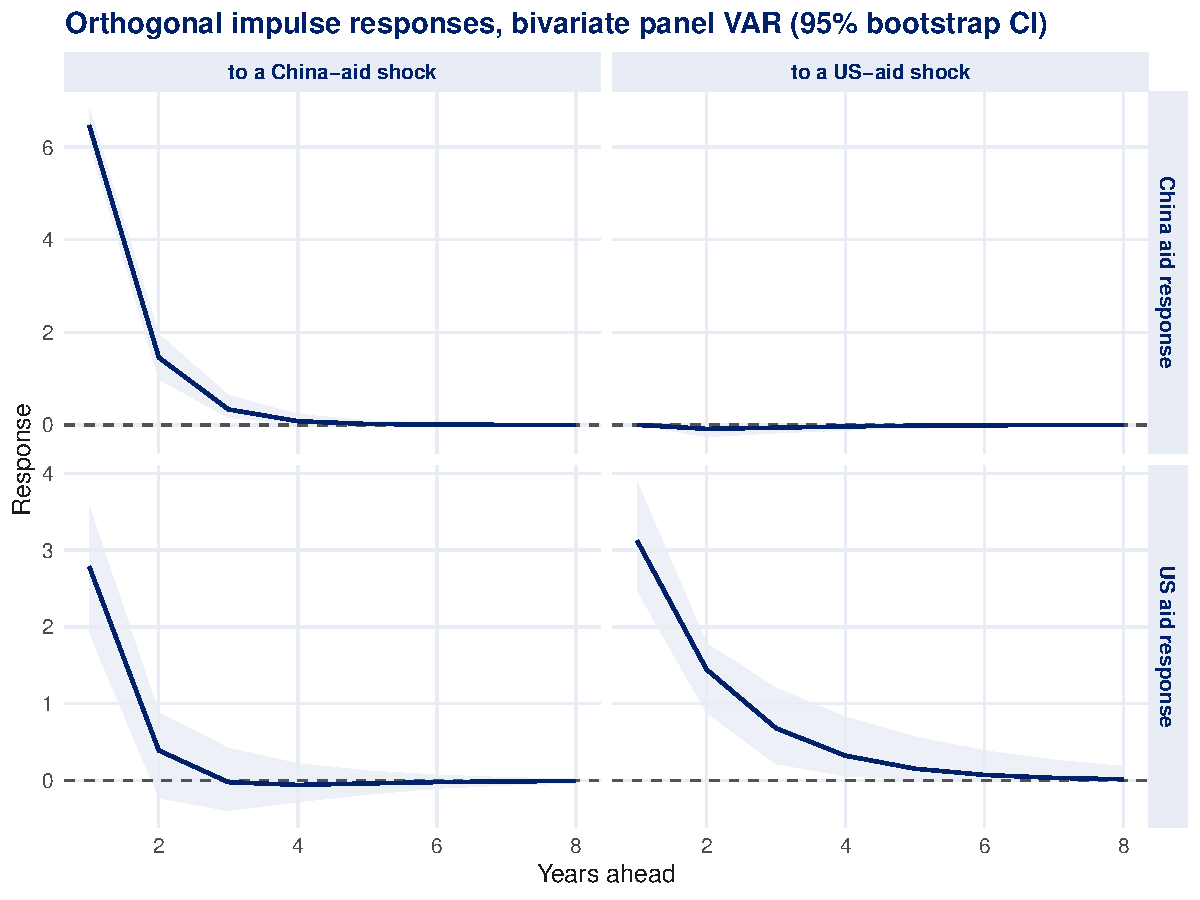
\includegraphics{fig_irf}         %% source: analyses/04_var_dynamics/scripts/R/05_figures.R

\section{Robustness}
\label{sec:quant-robustness}
\textit{Placeholder.} Specification curve / multiverse, leave-one-out by region,
alternative clustering and inference (per the project's inference-robustness
conventions).
